\chapter{Motivation}

This Bachelor thesis documents a part of the Bachelor project G1 2012 at the Hasso Plattner Institute in Potsdam. To support the documentation of innovative projects, a group of six students developed a software tool for the Hasso Plattner Institute School of Design Thinking (D-School) \footnote{\url{http://www.hpi.uni-potsdam.de/d_school/home.html?L=1}, accessed 06/16/13}. 

\section{Design Thinking at Hasso Plattner Institute}
The School of Design Thinking offers academic courses for students. Design Thinking is a method for creating new ideas and developing novel solutions \cite{Plattner_2009}. 

During the courses, students work on team projects. Starting in the Basic Track there are 1-week, 3-week and 6-week projects. In the Advanced Track students work 12 weeks continuously on one project. In addition to the students tracks the D-School also offers Executive Training where the projects usually don't exceed one week in length. 

As one of its core principles the D-School actively encourages multidisciplinary teams. This mixture of different background leads to multiple viewpoints during the design phases and helps the team to filter out obstacles early in the process. 

\begin{figure}[!h]
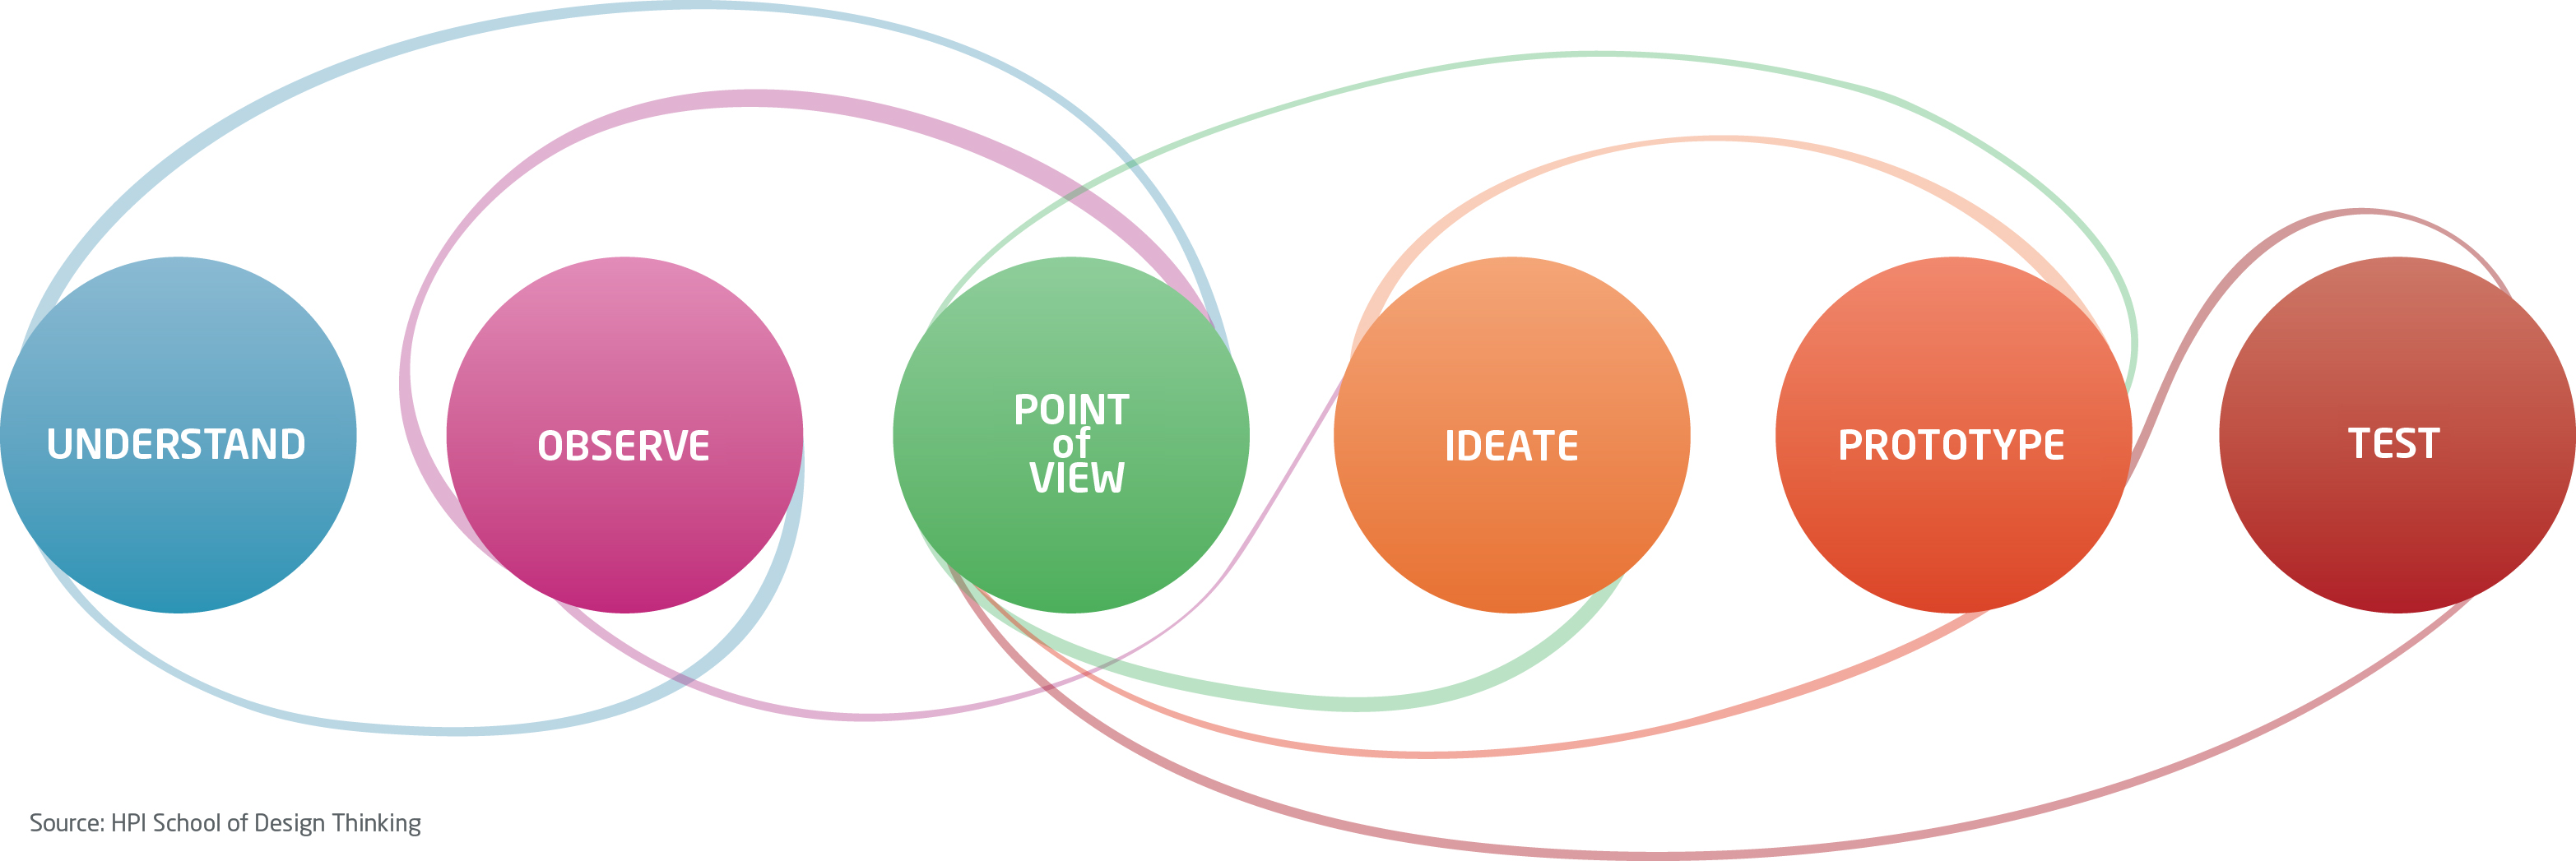
\includegraphics[width=\textwidth]{HPI_School_of_Design_Thinking_-_Prozess_en.jpg}
\caption{An overview of the phases in the Design Thinking process. Source: \cite{Plattner_2009}}
\label{fig:DT_phases}
\end{figure}

The projects usually deal with a problem posed by an industry partner. The Design Thinking method includes an iterative process which consists of several well-defined phases, shown in figure \ref{fig:DT_phases}. The phases guide the teams from basic understandings to the development of testable prototypes. The process is non-linear because the teams are encouraged to iterate. These cycles help to refine the prototypes based on actual user feedback. Throughout the process teachers are advising the students.
The D-School provides several team workspaces. A typical workspace consists of a set of whiteboards and a standing desk, which is large enough for the whole team to work on. The D-School considers open spaces to be important for the creative process, so the equipment is usually movable. Therefore, the spaces are hosted in large halls. The D-School also provides tools and materials for rapid prototyping.

There are several staff members at the D-School for coordinating and acquiring the student's pro\-jects. Key stakeholders for this thesis are the Head of D-School, the Program Manager, the Knowledge Manager and the Track Managers.

\section{Design process}
The Bachelor project also applied an iterative process, which is very similar to the one taught at the D-School. With this approach the project participants were able to benefit from the Design Thinking method while automatically learning about some of the needs of the D-School students.

\begin{figure}
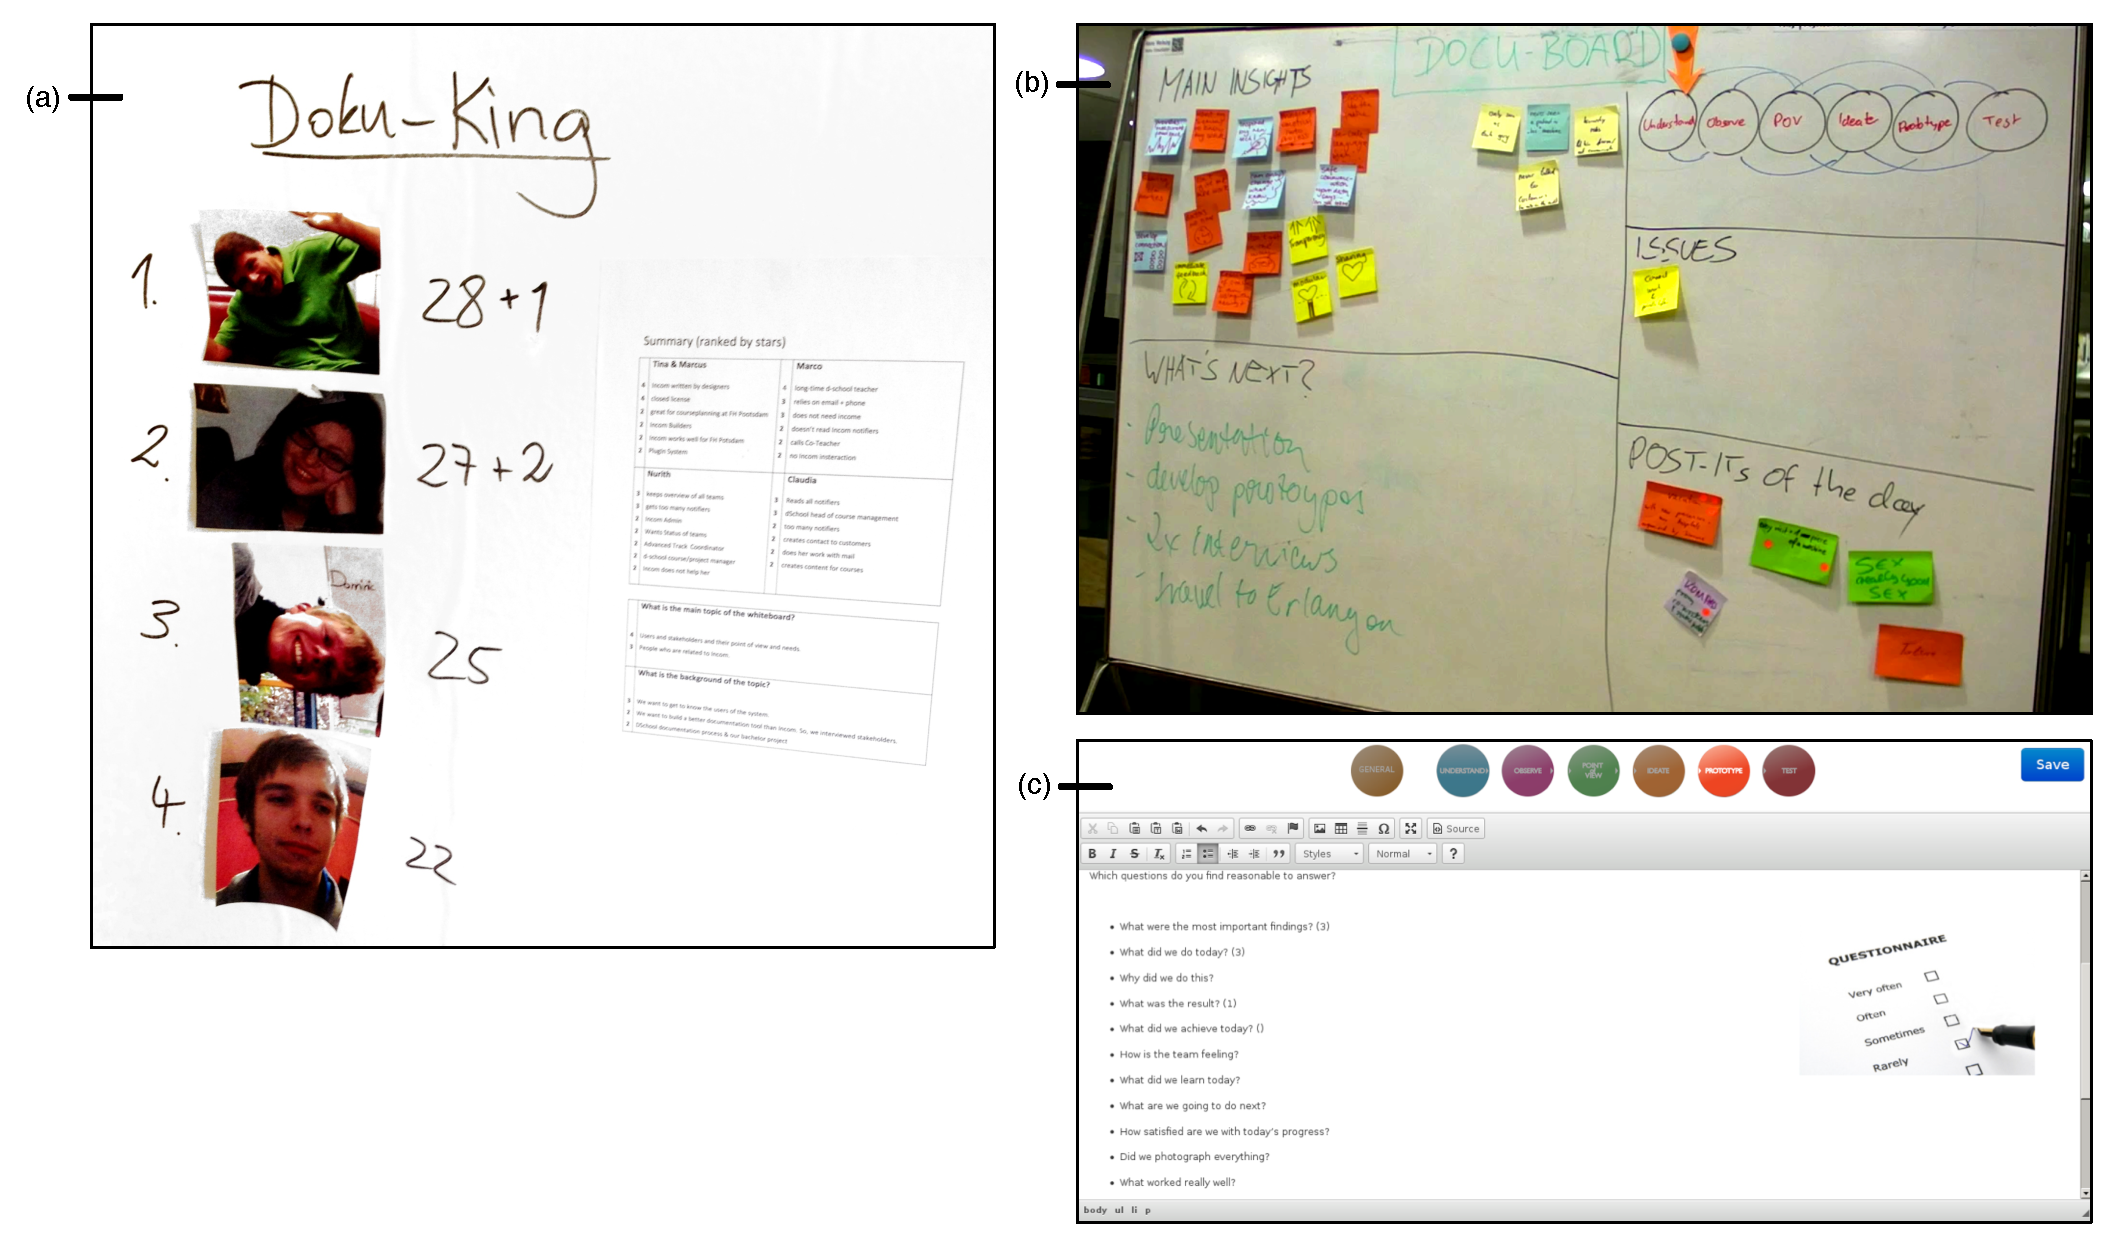
\includegraphics[width=\textwidth]{prototypes.pdf}
\caption[Prototypes created during the first design iteration]{Prototypes created during the first design iteration: \textit{(a)} Doku-King: a gamification\footnotemark ~approach, where players earn points by documenting their work and validating the results of others. \textit{(b)} Doku-Board: a preformatted white board, where students create daily summaries of the most important insights or results. \textit{(c)} a rich-text-based editor, where students can summarize their results structured by the Design Thinking phases.}
\label{fig:First_prototypes}
\end{figure}

\footnotetext{Gamification is a trend that connects concepts of human-computer-interaction and game studies. \cite{Deterding_2011}}

During the project there have been several interviews with the relevant stakeholders. The group learned about the student's documentation efforts, especially commonly used methods and tools. Other stakeholders like teachers or D-School staff members have also been interviewed. Based on this information, the prototypes shown in figure \ref{fig:First_prototypes} were developed to enhance the documenting experience of the students. These prototypes were evaluated during user testing sessions.

In the second iteration a new prototype was designed which also addressed the need of the staff members to archive and categorize the projects for easy retrieval. This prototype is called ``Project Zoom". The following sections will highlight the most relevant use cases and requirements for this thesis.\footnote{The ``Software Requirements Specification"\cite{ReqSpec} covers the use cases and requirements in detail.}

\subsection{Use Cases}
Project Zoom addresses two main use cases, which were distilled from the insights gathered in the observation phases.

\begin{labeling}{\textbf{R3:}}
\item[U1\label{uc:organize}] Student teams document their projects by organizing the digital documents they created, in a visual manner.\\
\textsc{Prerequisite}: The students have all documents they created digitally available.\\
\textsc{Postcondition}: A visual knowledge graph is being created.

\item[U2\label{uc:display}] D-School staff members get an overview of all projects. This overview enables access to the projects' classifications, related people and documentations.\\
\textsc{Prerequisite}: The projects were entered in a database (e.g. \textsc{Filemaker}\footnote{The D-School uses a \textsc{Filemaker} database to store projects and contacts. \url{http://www.filemaker.com/}, accessed 06/16/13}) and the students have documented their projects.\\
\textsc{Postcondition}: A visual representation of all projects is displayed.
\end{labeling}

Beyond these two major use cases there are other relevant use cases.

\begin{labeling}{\textbf{R3:}}

\item[U3\label{uc:fromhome}] The students add additional documents from their computers at home.\\
\textsc{Prerequisite}: The students have the documents digitally available. The computer needs to have an HTML5-capable web browser installed.\\
\textsc{Postcondition}: The documents are included in the knowledge graph.


\item[U4\label{uc:versions}] Students, teachers and D-School staff members can retrieve versions of the knowledge graph at different points in time.\\
\textsc{Prerequisite}: The students have documented their projects using the proposed tool.\\
\textsc{Postcondition}: A historical version of the knowledge graph is displayed.

\item[U5\label{uc:storageproviders}] Students can access the documents they saved using different commonly-used storage pro\-vi\-ders, e.g. \textsc{Box}\footnote{The D-School uses \textsc{Box} as a shared storage service. \url{https://www.box.com/}, accessed 06/16/13}.\\
\textsc{Prerequisite}: The students stored documents using the respective service.\\
\textsc{Postcondition}: Documents are offered for insertion in the knowledge graph.

\item[U6\label{uc:multiplatform}] The Head of D-School and Program Manager show an overview of a customizable set of pro\-jects to potential industry partners. \textit{Optional}:  A mobile tablet device is used for the presentation .\\
\textsc{Prerequisite}: The projects were entered in a database, e.g. \textsc{Filemaker}.\\
\textsc{Postcondition}: A visual representation of the projects is displayed.
\end{labeling}

\subsection{Requirements}

To fulfill these use cases there are some technical requirements for designing and implementing Project Zoom. The following is a selection of relevant requirements.

\begin{labeling}{\textbf{R3:}}
\item[R1\label{req:multiplatform}] The system's interface has to support multiple platforms, including the popular desktop operating systems and modern tablet devices. (use cases \ref{uc:fromhome}, \ref{uc:versions})
\item[R2\label{req:fromhome}] The system's interface has to be accessible from outside the D-School. (use case \ref{uc:fromhome})
\item[R3\label{req:concurrency}] The systems has to support concurrent users accessing and modifying contents. \textit{Simplifying assumption}: A resource (e.g. a project's graph) can only be modified by one user at the same time\footnote{Project teams at the D-School usually assign one member for documentation. Therefore, concurrent editing is not a high priority requirement.}. However, multiple users may edit different resources and any user can read any resource.
\item[R4\label{req:storageprovider}] The system connects to different data sources, e.g. \textsc{Box} and \textsc{Filemaker}, and makes the stored data available through its GUI. (use cases \ref{uc:organize}, \ref{uc:storageproviders})
\end{labeling}

\chapter{Application Design}
\section{User interface}
\label{sec:design}

Project Zoom is designed to apply the concept of semantic zooming. Semantic Zoom is part of the computer interface model \textsc{Pad} proposed by Perlin and Fox \cite{Perlin_1993}. This concept taps into the natural spatial thinking of users. Information is displayed on a large infinite two-dimensional canvas. Users browse around either by panning or zooming. There are different representations of the same pieces of information at different magnification levels. When zoomed out, documents are only represented by an icon or a title string. While zooming in, these abstract figures gradually resolve into the full representation of the respective documents. 

In Project Zoom there are three main zoom levels: An overview of all projects (\textbf{Overview view}), a detailed view of a project and its metadata (\textbf{Details view}), and a view containing a project's knowledge graph (\textbf{Process view}). Users can navigate from one view to the next by zooming in and out. This approach allows building one cohesive system, which hosts interfaces that are targeted at the specific needs of different stakeholders (see use cases \ref{uc:organize}-\ref{uc:storageproviders}). 

The main views themselves also support different zoom levels. Especially the Process view takes advantage of the zooming capabilities and displays the documents in the graph in different levels of detail. 
The Process view is an interactive graph that allows users to add documents onto the canvas and connect them with edges. The document nodes can then be annotate using the commenting feature or by drawing clusters (i.e. free form shapes) around them. These actions are exposed through context-sensitive menus. Also, the interactive graph features automatic layout capabilities, like collision prevention.

\section{Architecture}
In the design phase multiple architectures for Project Zoom have been evaluated. 

A \textbf{monolithic application} \footnote{Wikipedia, Monolithic application, \url{http://en.wikipedia.org/w/index.php?title=Monolithic_application&oldid=552899667}, accessed 06/17/13} is a self-contained system that can run on a single computer. The benefits are that the data is consistent for all users. Also, the system is easy to set up because there is only one computer required for the system to work. This approach is well suited for applications that deal with independent datasets, which can be stored on one platform. Word processors are an example of monolithic applications. However, as use cases \ref{uc:fromhome} and \ref{uc:versions} as well as requirements \ref{req:multiplatform} and \ref{req:concurrency} require the data to be accessible on multiple platforms concurrently this architectural approach isn't suitable for Project Zoom.

The \textbf{peer-to-peer} \cite{Schollmeier_2001} architecture allows the distribution of data on multiple connected computers. Each node in the network is equally privileged and handles a subset of the data individually. Data consistency can be eventually achieved through replication from on neighbor node to another. This is a well-known database problem \cite{Gray_1996}. Access control can be integrated by using trusted computing technology \cite{Sandhu_2005}. Peer-to-peer architectures are usually applied when a centralized controlling instance is to be avoided. Bitcoin\footnote{Bitcoin, \url{http://bitcoin.org/}, accessed 06/25/13} is a popular peer-to-peer application. The ability of a node to function, especially when joining the network, depends on the availability of neighbor nodes. Because of the low number of users the availability of nodes might pose as an issue in Project Zoom. Also, implementing a peer-to-peer usually requires to build a native application which makes it harder to fulfill requirement \ref{req:multiplatform}.

The \textbf{client-server} \cite{Berson_1996} model is one of the most-used distributed architectures. One central computer acts as a server, which stores the dataset and manages access control. Client computers can access and modify the resources on the server through a network interface. An example of a client-server application is the World Wide Web. Fundamentally, the server is a single point of failure\footnote{Wikipedia, Single point of failure, \url{http://en.wikipedia.org/w/index.php?title=Single_point_of_failure&oldid=555725127}, accessed 06/17/13}. However, there are methods to maximizing the availability \cite{Gray_1991} \cite{Colyer_2000}. This architecture is suitable for Project Zoom as it fulfills all the requirements, especially \ref{req:multiplatform}–\ref{req:concurrency}, and enables all the use cases.

A web-based client-server architecture is a system that uses an HTTP-Server \cite{RFC2616} and a brow\-ser application as client. Project Zoom incorporates this approach for several reasons:
\begin{itemize}
\item Using the client application of a web-based system only requires the installation of a web browser, which are wide-spread and usually preinstalled on the operating system. This makes it easy for students to modify the data from their computers at home (see: use case \ref{uc:fromhome}).
\item Developing native apps for mobile devices requires different technologies for each platform \cite{Charland_2011}. However, recent mobile devices are equipped with HTML5-capable \cite{W3C_HTML5} web browsers. Applications built using web technologies are likely to run on multiple mobile platforms (see: requirement \ref{req:multiplatform}).
\item Because of the standardization of the web technologies, emerging platforms will likely to support them as well.
\end{itemize}

Alternatives to web-based client-server architectures are based on client applications that users have to install on their devices. Because the users of Project Zoom use multiple computing devices, this isn't a favorable approach, as the application has to be installed on each device separately. Also, users may not even be able to install the application on to the device due to imposed access restrictions.

\begin{figure}
\begin{center}
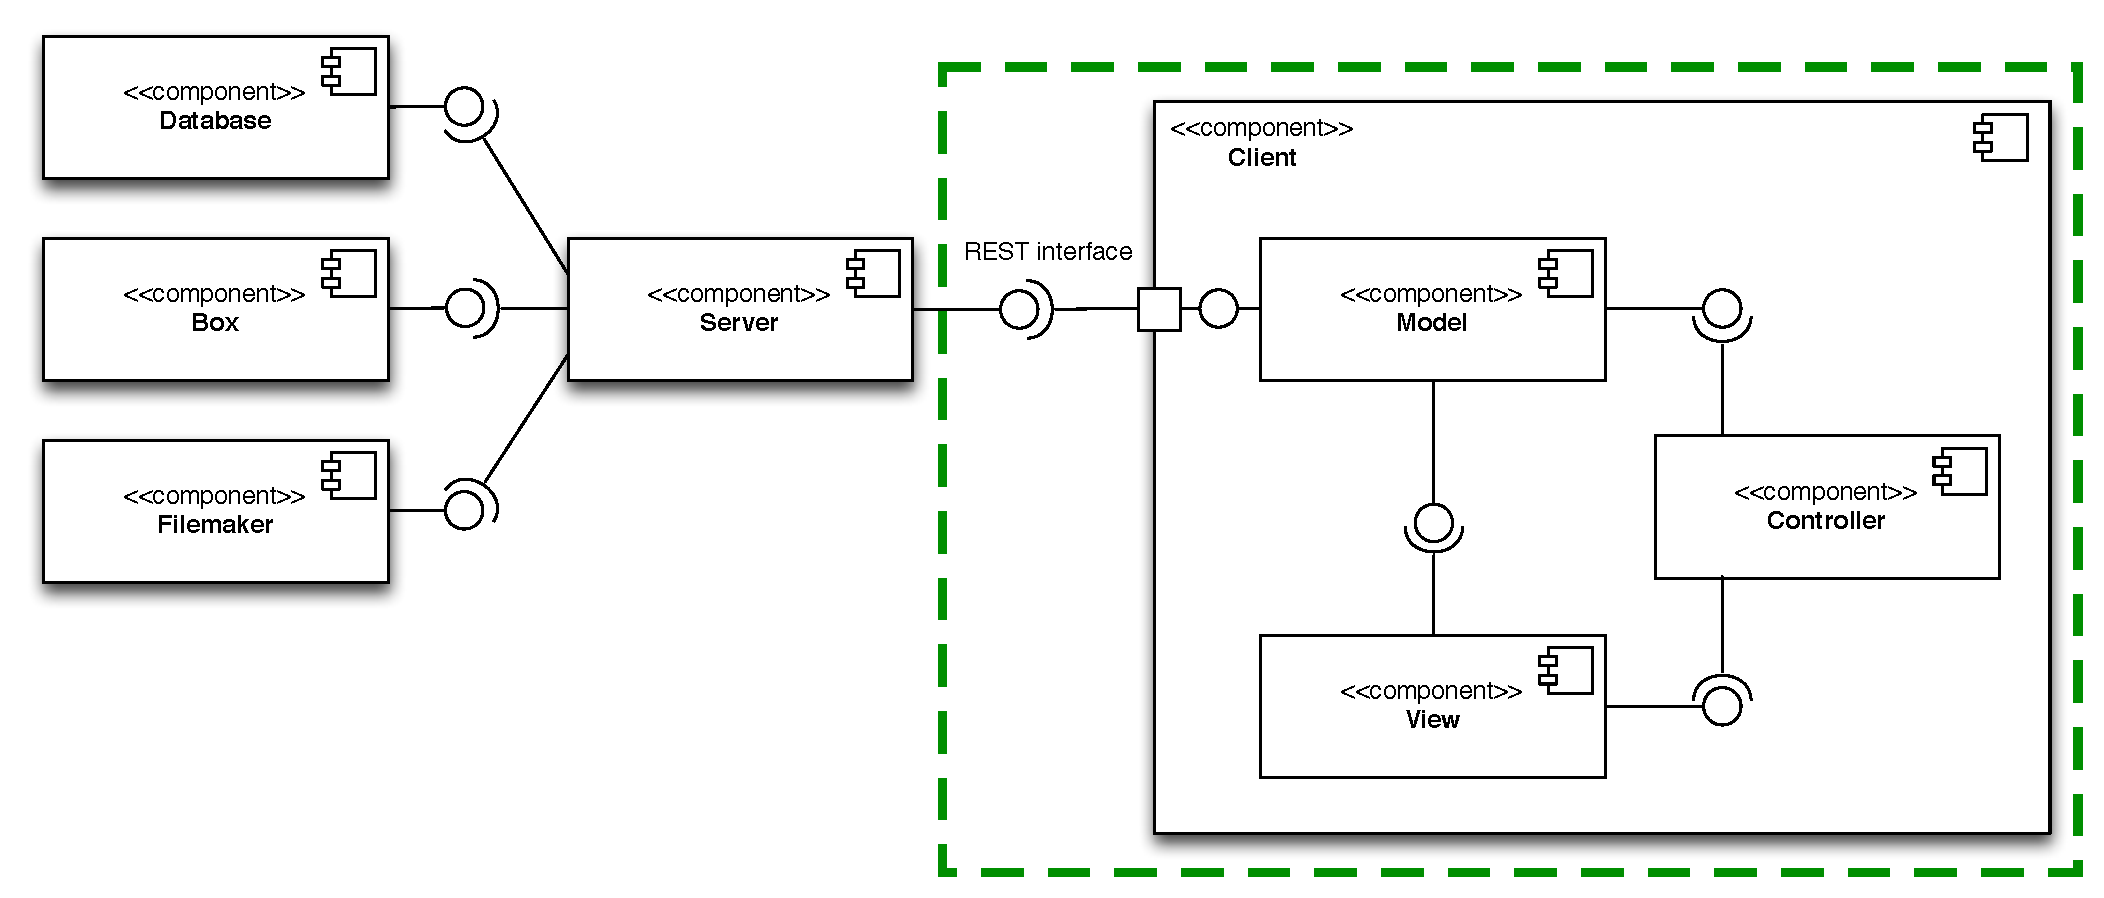
\includegraphics[width=0.7\textwidth]{architecture.pdf}
\caption{Architecture overview of Project Zoom. The highlighted part is covered by this thesis.}
\label{fig:CompleteArchitectureDiagram}
\end{center}
\end{figure}

Figure \ref{fig:CompleteArchitectureDiagram} shows the system architecture of Project Zoom. The server implementation features an event-system that is fed by the data connectors and sets up the pipeline for thumbnail generation. The server also hosts the database model and handles user access control and authentication. Client and server are connected through a REST interface \cite{Fielding_2000}. The client application is built using an MVC pattern, which will be detailed in later chapters. 

\section{Project context}
There are six theses covering Project Zoom. Bocklisch \cite{Bocklisch_2013} describes the architecture of the server and the domain data model. Werkmeister \cite{Werkmeister_2013} details the connection of the data pro\-vi\-ders, e.g. \textsc{Box} and \textsc{Filemaker}, to the system. Bräunlein's thesis \cite{Braeunlein_2013} covers both the design and generation of document thumbnails for the Process View. Dieckhoff \cite{Dieckhoff_2013} details the automatic layouting capabilities of the interactive graphs. Herold \cite{Herold_2013} explains the context-sensitive actions that users can perform on the graph and its nodes and edges. This thesis is about the architecture of the client application, as highlighted in figure \ref{fig:CompleteArchitectureDiagram}.

